\documentclass{article}
\usepackage{mathtools}
\usepackage[top=2in, bottom=1.5in, left=1in, right=1in]{geometry}
\usepackage{graphicx}
\usepackage[normalem]{ulem}
\usepackage{fancyhdr}
\usepackage{enumerate}
\pagestyle{fancyplain}

\lhead{PHYS 152 Section 10}

\rhead{A. Shawn Bandy 
(003635396)}


\begin{document}
\title{Lab 8:  Energy Storage and Release in Circuits}
\author{A. Shawn Bandy}
\date{March 26\textsuperscript{th}, 2013}
\maketitle
\begin{abstract}
In this lab, we explored the properties of resistor/capacitor circuits to see how energy is stored, delivered, and manipulated in a circuit.  We estimate the time constant of an arbitrary RC circuit.
\end{abstract}
\begingroup
	\section{Data and Data Tables}\hfill\\
		\let\clearpage\relax
			\begin{enumerate}[A.]
			\subsection{DATA SHEET \#1} 

	\item Calculate the time constant for the circuit with the above values of R and C.\\
		
		RC = 0.00015 seconds
	\item Record the frequency reading from the function generator.\\
	
		Calculate the period T for this wave: 600.3 Hz \\
		
	\item Record your vertical (VOLTS/DIV) and horizontal settings (TIME/DIV) for the capacitor channel CH2 in the boxes below.
	
		VOLTS/DIV = 1 V\\
		
		TIME/DIV = 0.5 ms.
	\begin{samepage}
	\item Draw carefully what you observe on the screen for the capacitor response at these settings.\\
	
		\includegraphics[width=300px]{lab8_graph1}
	\end{samepage}
	\item From the screen, what is the charging time for the capacitor in one cycle?\\
	
		1.5 divisions or about 0.8 ms.\\
	
	\item State how the screen image of a charging cycle is consistent or not with the time constant of this circuit.  Is the charging cycle much longer or much shorter than RC?\\
	
		The charging time is about 0.7 ms shorter on the screen than we calculated above.
	
		
			\subsection{DATA SHEET\#2}
	\item Watch the images on the screen as you do the following.  Keep C = 0.01 $\mu F$ on the capacitance box.  From the resistance decade box setting of the R = 10 $k \Omega$, rotate the knob to 20 $k \Omega$, 30 $k \Omega$, up to 50 $k\Omega$.  Describe what happens to the image on the screen.\\
	
	The vertical range for the charging curve contracts, pulling away from both the upper and lower square wave marks.\\
	
	\item At the R = 50 $k\Omega$ and C = $0.01 \mu F$ setting, what is the time constant?\\
	
	0.0005 seconds.
	
	\item Set R back to R = 10 $k \Omega$.  Now dial capacitance up to C = 0.05 $\mu F$  Describe what happens to the image on the screen.\\
	
	The vertical range for the charging curve contracts, pulling away from both the upper and lower square wave marks.\\
	
	\item At the R = 10 $k \Omega$ and C = 0.05 $\mu $ what is the time constant? \\
	
	0.0005 seconds
	
	\item Experimentally measure the time constant of an RC circuit using the oscilloscope.\\
		\begin{enumerate}[1.]
			\item Choose to set the capacitance to some value C between 0.02 $\mu F$ and 0.01 $\mu F$.\\
			
			
			Record the value of $C \pm 5\%$ uncertainty = $ 0.021 \mu F \pm 0.00105 \mu F$\\
			
			\item  Choose to set the resistance to some value R between 2 $k \Omega$ and 9 $k \Omega$\\
			
			Record the value of $R \pm 1 \%$ uncertainty = $ 5 \pm  0.05 k \Omega$\\
			
			\item Compute the time constant of this combination, appropriately propagating the uncertainties.  In order to come out in units of seconds, you have to multiply ohms x farads.\\
			
			RC = $ 0.000105 \pm  0.050011 seconds$\\
			
			\item Because the mathematical description of a discharging C is a little simpler, namely $ \Delta V_c(t) = \Delta V_{batt}(e^{-\frac{t}{RC}})$, set the oscilloscope to trigger on the negative slope of the discharge cycle, and then measure on the screen the time that a discharging capacitor will take to reach 37\% of its initial voltage.  The next steps will indicate how to set the trigger to negative slope in order to observe the char charge cycle first.
			\subsection{DATA SHEET \#3}
		\item Get several cycles on the screen by increasing or decreasing the frequency of the square wave from the function generator, and record that frequency below.  You want to set the frequency so that the charging and discharging cycle just reaches the maximum and minimum values, respectively (about 4 time constants wide).\\
		
		$f_1 = 813.6$  cycles per second\\
		
		\item Display only the capacitor waveform by setting the MODE switch to CH2.\\
		
		\item Push in GND for CH2 and use the vertical position adjust to center the beam trace on the screen.  Then make sure the COUPLING is set back to DC and the capacitor waveform is on the screen.\\
		
		\item Once the capacitor waveform is back on the screen, the goal is to get the heigh of one cycle to fill the full vertical eight (8) divisions on the screen.  The reason is purely practical:  we want to experimentally determine the time constant,  when the value of the voltage falls to about 37\% of its maximum.  If the maximum value of voltage is 8 divisions, then 0.37 * 8 = 2.96 $\approx$ 3.  So the time constant measured on the screen is simply the number of horizontal divisions from the left to where the voltage crosses into that $3^{rd}$ vertical DIV.
		
		\begin{enumerate}[a.]
			\item Adjust the CH2 VOLTS/DIV control to extend the vertical waveform height to beyond the 8 division vertical range.  Then use the central CAL knob to adjust the height downward until waveform just fits into the.  For this purpose it is OK to remove the calibration from the vertical scale, because the scaling is proportional and maintains the relationship between the maximum and the 0.37 of the maximum.\\
			
			\item On the TRIGGER LEVEL control, pull out the central knob to trigger on the negative slope of the discharge part of the cycle.\\
			
			\item Adjust the HORIZ POSITION to set the leftmost part of the signal at the top left corner of the display.\\
			
			\item Then adjust the TIM/DIV knob to spread the discharge line as widely as possible along the horizontal axis, while still being able to see where ethe descending voltage crosses the ? to ? of the $3^{rd}$ vertical division.\\
			
			\item As precisely as possible, count and record below the number of divisions horizontally from the left edge to the crossing point described above.  For example, in the picture above, that is 3.9 DIV.
		\end{enumerate}
		
		\item \# of time divisions for voltage to drop to 0.37 * max = $ 1.2 \pm 0.05$\\
		
		\item TIME/DIV SETTING = 20 microseconds\\
		
		\item TIME CONSTANT (EXP. MEASUREMENT) = $ 24  \pm 0.05$ microseconds\\
		
	\end{enumerate}
			\subsection{DATA SHEET \#4}
			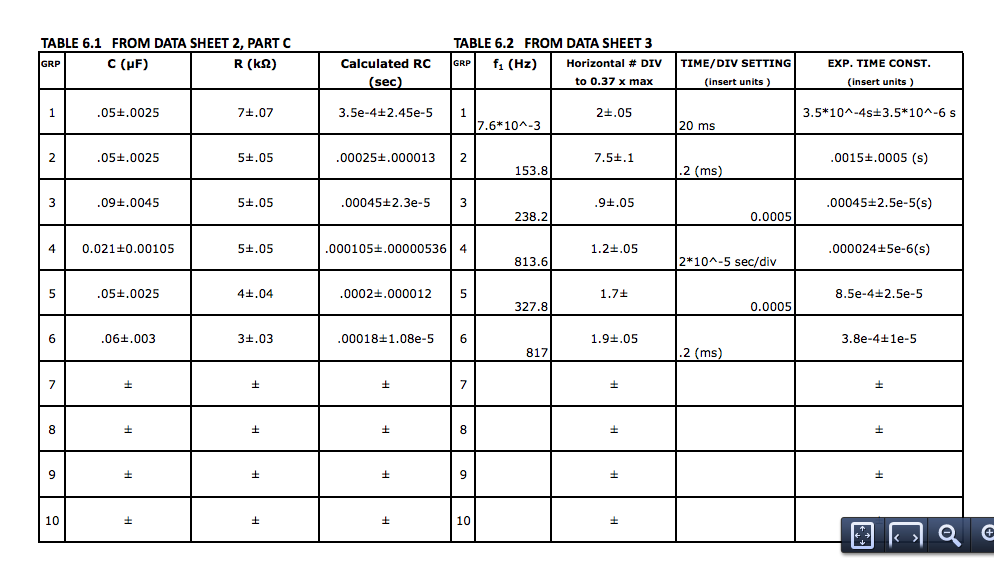
\includegraphics[width=500px]{lab8_table1}
			\end{enumerate}
\endgroup
\begingroup
	\section{Graphs and Diagrams}\hfill\\
			See Data Tables sections\\
			

\endgroup
\begingroup
	\section{Uncertainty Calculations}\hfill\\
		\let\clearpage\relax
			See Data Tables sections\\
\endgroup
\begingroup
	\section{Results}\hfill\\
		We estimate the time constant of the circuit at 24 $\pm$ microseconds.
\endgroup
\begingroup
	\section{Discussion}\hfill\\
		\let\clearpage\relax
			
We assembled the circuit as described in the lab manual with a function generator , a variable capacitance box, a variable resistance box and to both channels on a 2-channel oscilloscope.   We began by setting the capacitance box to $0.01 \mu F$ and the resistance box to $10 k\Omega$.  We began with the function generator set to produce square waves at 600 Hz and the oscilloscope with the settings described in the lab manual.  This produced the a display on the oscilloscope as seen on Data Sheet \#1 part D.  Next we altered the values for the resistor and capacitance and found that for a given RC, the resulting display was the same without respect to the individual settings for R or for C.  We then set about measuring the time constant of an RC circuit by taking measurements from the oscilloscope.  We adjusted the display so that the height of one cycle filled the 8 divisions.  The time constant is the interval it takes for the voltage to fall to about 37\% of its maximum or where it crosses the 3 vertical division from the bottom.  We estimate that this occurred at 1.2 horizontal divisions and the TIME/DIV was set to 20 microseconds so the time constant was 24 microseconds.\\

As with all of these experiments error in our measurements occurred in three categories.  The first type is error in actually taking the measurements.  For example, we could only reasonably estimate the a given point on the oscilloscope to within one half tick marks.  Second, given the number of leads and the age of the capacitor and resistor boxes, there could be noise or false measurements that we cannot anticipate in our measurements.  Third, we make assumptions to simplify the physics involved in the circuits:  for example, we do not measure the resistance of the leads.\\
\endgroup
\begingroup
	\section{Questions and Answers }\hfill\\
		See Data Tables sections
\endgroup
\end{document}